\documentclass[12pt,answers]{exam} 
\usepackage{ctex}
\usepackage{amsmath}
\usepackage{graphicx}
\graphicspath{{fig/pdf/}}
\usepackage{caption}
\usepackage[T1]{fontenc}
\usepackage{fourier}
\usepackage{amssymb}
\usepackage{gensymb}
\usepackage{xeCJK} 
\setCJKmainfont{SimSun}
\setCJKmonofont{SimSun} 
\setmainfont{Times New Roman} 

%\setmainfont{SimSun}


\renewcommand{\thepartno}{\arabic{partno}}
\renewcommand{\solutiontitle}{\noindent\textbf{解:}\par\noindent}
%\newcommand{\solutiontitle}{\noindent\textbf{Solution:}\enspace}
%\title{正切函数的图像与性质}
%\date{}
\begin{document}
%\maketitle
\heiti{6.2\quad 正切函数的图像与性质}
\begin{questions}
\question 
\begin{parts}
\part 求函数$y=\tan{\frac{x}{a}}$ 的最小正周期
\begin{solution}
因为 $\tan{x}$ 的周期为$\pi$,所以 有 $\frac{\pi}{\frac{1}{|a|}} = |a|\pi$
\end{solution}
\part 求函数$y=\tan{x}-\cot{x}$ 的最小正周期
\begin{solution}
$y=\frac{\sin{x}}{\cos{x}} -\frac{\cos{x}}{\sin{x}} =-2\frac{\cos{2x}}{\sin{2x}}=-2\cot{2x}$ 
最小正周期为$\frac{\pi}{2}$
\end{solution}
\end{parts}
\question 下列不等式中成立的是? \fillin[B]
\\
\begin{oneparchoices}
\choice $\tan(1) < \tan(4)$ 
\CorrectChoice $\cot(1) < \cot(4)$
\choice $\sin(1) < \sin(4)$
\choice $\cos(1) < \cos(4)$
\end{oneparchoices}
\begin{solution}
注意到 $\sin{(1)}>0$,$\sin{(4)}<0$以及$\cos{(1)}>0$,$\cos{(4)}<0$ 可以知道 $C,D$ 错误\\
由于 $\tan{(4)}=\tan{(4-\pi+\pi)}=\tan{(4-\pi)}<\tan{(1)}$ 故$A$ 错 \\
$\cot{(4)}=\cot{(4-\pi+\pi)}=\cot(4-\pi)>\cot{(1)}$ 

\end{solution}

\question 求函数$y=\tan(3x+\frac{\pi}{4})$的单调递增区间
\begin{solution}
\[k\pi-\frac{\pi}{2}< 3x+\frac{\pi}{4}< k\pi+\frac{\pi}{2},k\in Z\]
\[ x\in (\frac{k\pi}{3}-\frac{\pi}{4},\frac{k\pi}{3}+\frac{\pi}{12} ),k \in Z\]
\end{solution}

\question 求函数 $y=\tan(2x-\frac{\pi}{4})$的对称中心
\begin{solution}
先求 $y=\tan{x}$ 的对称中心 ,设对称中心为$(a,0)$
根据对称中心的定义,应该有 f(x)+f(2a-x)=0,由此可知 $2a=k\pi$,即
$y=\tan{x}$ 的对称中心为 $(\frac{k\pi}{2},0),k\in Z$
因此只需要
\[2x-\frac{\pi}{4} =\frac{k\pi}{2}\]
即 \[x=\frac{k\pi}{4} +\frac{\pi}{8}\]
即对称中心为$(x=\frac{k\pi}{4} +\frac{\pi}{8},0),k\in Z$
\end{solution}

\question 
\begin{parts}
\part 函数$y=\tan(|x|)$的图像关于\fillin[$x=0$] 对称
\part 函数$y=\tan{x} +\cot{x}$ 的奇偶性是 \fillin[奇函数]
\end{parts}
\question
在下列函数中,同时满足:(1) 在$(0,\frac{\pi}{2})$ 上递增;
(2) 以$2\pi$为 最小正周期; (3)为奇函数的函数是\fillin[C]\\
\begin{oneparchoices}
\choice $y=\tan{x}$ 
\choice $y=\cos{x}$
\CorrectChoice $y=\tan{\frac{x}{2}}$ 
\choice $y=-\tan{x}$
\end{oneparchoices}
\question 
求下列函数的定义域
\begin{parts}
\part $\tan{x}\cdot \cot{x}$
\begin{solution}
定义域是$\tan{x}$的定义域和 $\cot{x}$ 定义域的交
$\{x|x\in R,x\ne \frac{k\pi}{2},k\in Z \}$
\end{solution}
\part $y=\frac{1}{1+\tan{2x}}$
\begin{solution}
1. $\tan{2x}\ne-1\Longrightarrow x\ne -\frac{\pi}{8}+\frac{k\pi}{2}$ \\
2. $x\ne \frac{\pi}{4}+\frac{k\pi}{2}$ 
因此定义域为 $\{x|x\in R,x\ne -\frac{\pi}{8}+\frac{k\pi}{2} \text{且} x\ne \frac{\pi}{4}+\frac{k\pi}{2},k\in Z \}$

\end{solution}
\part $y=\lg(\tan{x}+1)$
\end{parts}
\begin{solution}
1. $\tan{x}+1>0 \Longrightarrow x\in(-\frac{\pi}{4}+k\pi,\frac{\pi}{2}+k\pi)$ 
\end{solution}
\question 
\begin{parts}
\part 函数$y=\tan{(\frac{\pi}{3}-x)}$,$x\in[0,\frac{\pi}{3}]$ 的值域是\fillin[[$0$,$\sqrt{3}$]]
\part 已知 $x\in [-\frac{\pi}{6},\frac{\pi}{4}]$,求函数 $y=\sec^2{x}+\tan{x}+2$ 的值域
\begin{solution}
\begin{equation*}
\begin{split}
y&=\frac{1}{\cos^2{x}}+\tan{x}+2 \\
 &=\frac{\sin^2{x}+\cos^2{x}}{\cos^2{x}}+\tan{x}+2\\ 
& = \tan^2{x}+\tan{x} +3 \\
&= (\tan{x}+\frac{1}{2})^2 + \frac{11}{4}\\
\end{split}
\end{equation*}
由于$x\in [-\frac{\pi}{6},\frac{\pi}{4}]$,可知$\tan{x}\in [-\frac{\sqrt{3}}{3},1]$,
所以 $y\in[\frac{11}{4},5]$
\end{solution}

\end{parts}
\question 
函数$y=a\tan{x}+b$ 在区间$[k\pi-\frac{\pi}{3},k\pi+\frac{\pi}{3}]$ 的最大最小值分别为$\sqrt{3}+1,\sqrt{3}-1$,求实数a,b
\begin{solution}
\begin{equation*}
\begin{split}
\sqrt{3}a+b&=\sqrt{3}+1 \\
-\sqrt{3}a+b &=\sqrt{3}-1
\end{split}
\end{equation*}
$$\Longrightarrow b=\sqrt{3},a=\frac{\sqrt{3}}{3}$$
或者
\begin{equation*}
\begin{split}
\sqrt{3}a+b&=\sqrt{3}-1 \\
-\sqrt{3}a+b &=\sqrt{3}+1
\end{split}
\end{equation*}
$$\Longrightarrow b=\sqrt{3},a=-\frac{\sqrt{3}}{3}$$
\end{solution}

\question $y=\sin{x}$与$y=\tan{x}$ 的图像在$[-2\pi,2\pi]$ 的交点个数为\fillin[5]
\ifprintanswers
\begin{figure}[!h]
\begin{center}
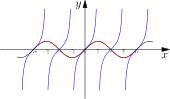
\includegraphics{intersect.pdf}
\end{center}
\caption{$y=\sin{x} $ 和 $y=\tan{x}$ 图像}
\end{figure}
\fi
\begin{solution}
只需要 求$\sin{x}=\tan{x}$ 在$[-2\pi,2\pi]$ 上的根的个数即可\\
即 $\cos{x}=1$ 或者$\sin{x}=0$ 
\end{solution}
\question 
直线 $y=a$ 与正切函数$y=\tan{\omega x},\omega>0$ 图像相邻两个交点间的距离为 \fillin[$\frac{\pi}{\omega}$]
\begin{solution}
设相邻的两个点为$(x_1,a),(x_2,a)$ 问题要求的是 $|x_1-x_2|$,因为$\tan{\omega x}$在所属的一个周期里单调,出现相等只能发生在两个周期之间,所以$|x_1-x_2|$ 等于 $\tan{\omega x}$的最小正周期 $\frac{\pi}{\omega}$
\end{solution}
\question
函数 $y=A\tan(\omega x +\phi),A>0,\omega>0,|\phi|<\frac{\pi}{2}$的图像与$x$轴相交的两相邻点坐标分别为
$(\frac{5\pi}{6},0),(\frac{\pi}{6},0)$,且经过点$(0,-3)$,求函数表达式。
\begin{solution}
由 $T=\frac{5\pi}{6}-\frac{\pi}{6}=\frac{2\pi}{3}$ 得
\[\omega=\frac{\pi}{T}=\frac{3}{2}\]
将$(\frac{\pi}{6},0)$ 代入 得$$\phi=-\frac{\pi}{4}$$
将$(0,-3)$ 代入 得$$A=3$$
所以 函数为$y=3\tan{(\frac{3}{2}x-\frac{\pi}{4})}$
\end{solution}
\question
如图,墙上有一壁画,最高点$A$离地面高$4$米
,最低点$B$ 离地面2米,观察者从距离墙$x(x>1)$ 米,离地面高
$a(1\le a\le 2)$米的$C$处观赏该壁画,设观赏视角$\angle ACB=\theta$ 
%\begin{figure}[!htbp]
\begin{center}

\includegraphics{wall.pdf}
\end{center}
%\end{figure}
\begin{parts}
\part 若$a=1.5$,问:观察者离墙多远时,视角$\theta$最大?
\begin{solution}
设$\theta_1=\angle{BCD},\theta_2=\angle{ACD}$,则$\tan{\theta_1}=\frac{2-a}{x}$,$\tan{\theta_2}=\frac{4-a}{x}$ 
而 $\theta=\theta_2-\theta_1$ 
由 \[\tan{\theta}=\tan{(\theta_2-\theta_1)} =\frac{\tan{\theta_2}-\tan{\theta_1}}{1+\tan{\theta_1}\tan{\theta_2}}= \frac{\frac{2}{x}}{1+\frac{(2-a)(4-a)}{x^2}}=\frac{2x}{x^2+(2-a)(4-a)}\]
当$a=1.5$ 时,$\tan{\theta}=\frac{2x}{x^2+1.25},x>1$.
因为 \[\frac{1}{\tan{\theta}} =\frac{1}{2}(x+\frac{1.25}{x})\ge \sqrt{1.25}\]
可得 $\tan{\theta}\le \frac{1}{\sqrt{1.25}}$
\end{solution}
\part 若$\tan{\theta}=\frac{1}{2}$,当$a$变化时,求$x$的取值范围?
\begin{solution}
当$\tan{\theta}=\frac{1}{2}$时
\[(x-2)^2=4-(2-a)(4-a),1\le a\le 2\]
可知 $4-(2-a)(4-a) \in [1,4]$, $\Longrightarrow x\in[3,4]$
\end{solution}
\end{parts}
\question
一幢高楼上安放了一块高约10米的LED广告屏,一测量爱好者在与高楼底部同一水平线上的C处测广告屏顶端A处的仰角为31.80度,再向大楼前进20米到D处,测得广告屏顶端A处的仰角为37.78度,人的高度忽略不计:
\begin{center}

\includegraphics{led.pdf}
\end{center}
\begin{parts}
\part 求大楼的高度(从地面到广告屏顶端)(精确到1米)
\begin{solution}
设 房高AE为$y$,D距离房子距离DE为$x$,则有
\begin{equation*}
\begin{split}
\frac{y}{x} =&\tan{(37.78^{\degree})} \\
\frac{y}{x+20}=&\tan{(31.80^{\degree})}
\end{split}
\end{equation*}
$\Longrightarrow y=61.97$
\end{solution}
\part 若大楼的前方是一片公园空地,空地上可以安放一些长椅,为使坐在其中一个长椅上
的观看广告最清晰(长椅的高度忽略不计),长椅需安置在距大楼底部E 处多远?已
知视角$\angle{AMB}$(M 为观测者的位置,B为广告屏底部)越大,观看得越清晰.
\end{parts}
\begin{solution}
设 距离为$x$, $\tan{\angle{AMB}}=\tan{(\angle{AME}-\angle{BME})}$,则
\begin{equation*}
\begin{split}
y&=\tan{\angle{AMB}}\\
 &=\frac{\tan{\angle{AME}}-\tan{\angle{BME}}}{1+\tan{\angle{AME}}\tan{\angle{BME}}} \\
&= \frac{\frac{62}{x}-\frac{52}{x}}{1+\frac{62*52}{x^2}}\\
& =\frac{10x}{x^2+3224} \\
&=\frac{10}{x+\frac{3224}{x}}\le \frac{5}{\sqrt{3224}}
\end{split}
\end{equation*}
$\Longrightarrow x=\sqrt{3224}$
\end{solution}
\end{questions}
\end{document}